% !TEX encoding = UTF-8 Unicode
% -*- coding: UTF-8; -*-
% vim: set fenc=utf-8

\section{Algoritmy používané pro kolaborativní editaci textů}\label{sec:algoritmyProKolaborativníEditaci}

Synchronizace dvou a více kopií stejného dokumentu ve skutečném čase je komplexní problém.
V této sekci popisuji přístupy k synchronizaci textů, ale také dva nejznámější a nejrozšířenější algoritmy pro synchronizaci textu mezi více klienty při použití architektury klient-server~\cite{algoritmy:first}.

\subsection{Druhy algoritmů}\label{subsec:druhyAlgoritmů}

Existují tři nejčastější přístupy k problému synchronizace, metoda zamykání (nebo také vlastnictví), předávání událost a třísměrné sloučení.

Metoda \textbf{zamykaní} je nejjednodušší technika.
Ve své nejčastější formě může dokument v jednu chvíli editovat pouze jeden uživatel a to ten který si dokument uzamkl.
Ostatní uživatele mohou dokument pouze číst.
Provádět změny mohou pouze po uvolnění zámku, stažení nové verze dokumentu a přivlastnění jeho zámku.

Některé vylepšené algoritmy na základě uzamykání se pokoušejí automaticky uzamykat pouze upravované části dokumentu.
To však zamezuje úzké spolupráci více uživatelů nad dokumentem, protože každý může pracovat pouze na své uzamčené části.

Metoda \textbf{předávání událostí} spočívá v myšlence zachycení všech změn provedených nad dokumentem a jejich provedení nad všemi kopiemi zároveň.
Hlavní představitelem tohoto přístupu je právě operační transformace, o které píší níže v sekci~\ref{subsec:operacniTransformace}.

Hlavním problémem tohoto přístupu je zachycení všech změn dokumentu, které mohou být triviální, jako je například napsání znaku, ale také například vložení obrázku, přetažení velkého množství textu, automatická oprava překlepů a mnoho dalších.
Přístup předávání událostí není přirozeně konvergentní.
Každá změna, která není správně zachycena (nebo ztracena při cestě po síti), vytváří novou verzi dokumentu, kterou již není možné správně obnovit.

Poslední častou metodou je takzvané \textbf{třísměrné sloučení}.
Uživatel odešle svůj změněný dokument na server, který provede sloučení s aktuální verzí na serveru a uživateli pošle novou sloučenou verzi zpět.
Pokud uživatel provedl v době synchronizace v dokumentu změny novou verzi ignoruje a musí se o synchronizaci pokusit znovu později.

Jedná se poloduplexní systém, dokud uživatel píše nedostává žádné aktualizace o dokumentu a ve chvíli, co psát přestane, se všechny změny od ostatních uživatel zobrazí nebo se zobrazí hláška o nastalé kolizi (to záleží na použitém slučovacím algoritmu).~\cite{ds:neil_paper}~\cite{ds:neil_video}

\enquote{\textit{Tento systém lze přirovnat k automobilu s čelním sklem, které se stane během jízdy neprůhledné.
Podívej se na cestu, pak jeď chvilku poslepu, pak zastav a podívej se znovu.
Kdyby všichni řídili stejný druh \enquote{dívej se, anebo jeď} automobilů, těžké nehody by byly velmi časté.}}~\cite{ds:neil_paper} přeložil Jiří Šimeček

Příkladem systému, který používá třísměrné sloučení, je například \gls{SVN}, systém pro správu zdrojových kódů.

\subsection{Diferenciální synchronizace}\label{subsec:diferencialniSynchronizace}

\gls{DS} je algoritmus, který vymyslel Neil Fraser a lze považovat za zástupce třísměrného sloučení.
\gls{DS} řeší problém s průběžnou synchronizací, kterým trpí klasický model třísměrného sloučení, a to použitím stínových kopií a diff-patch algoritmu nejen na serveru, ale i u každé kopie dokumentu.

Na obrázek číslo~\ref{fig:DS_diagram} je vidět zjednodušený vývojový diagram \gls{DS} algoritmu.
Diagram předpokládá dva dokumenty (pojmenované server text a klient text), které jsou umístěné na stejném počítači a tedy nepočítá se síťovou dobou odezvy.

\begin{figure}[ht]
    \centering
    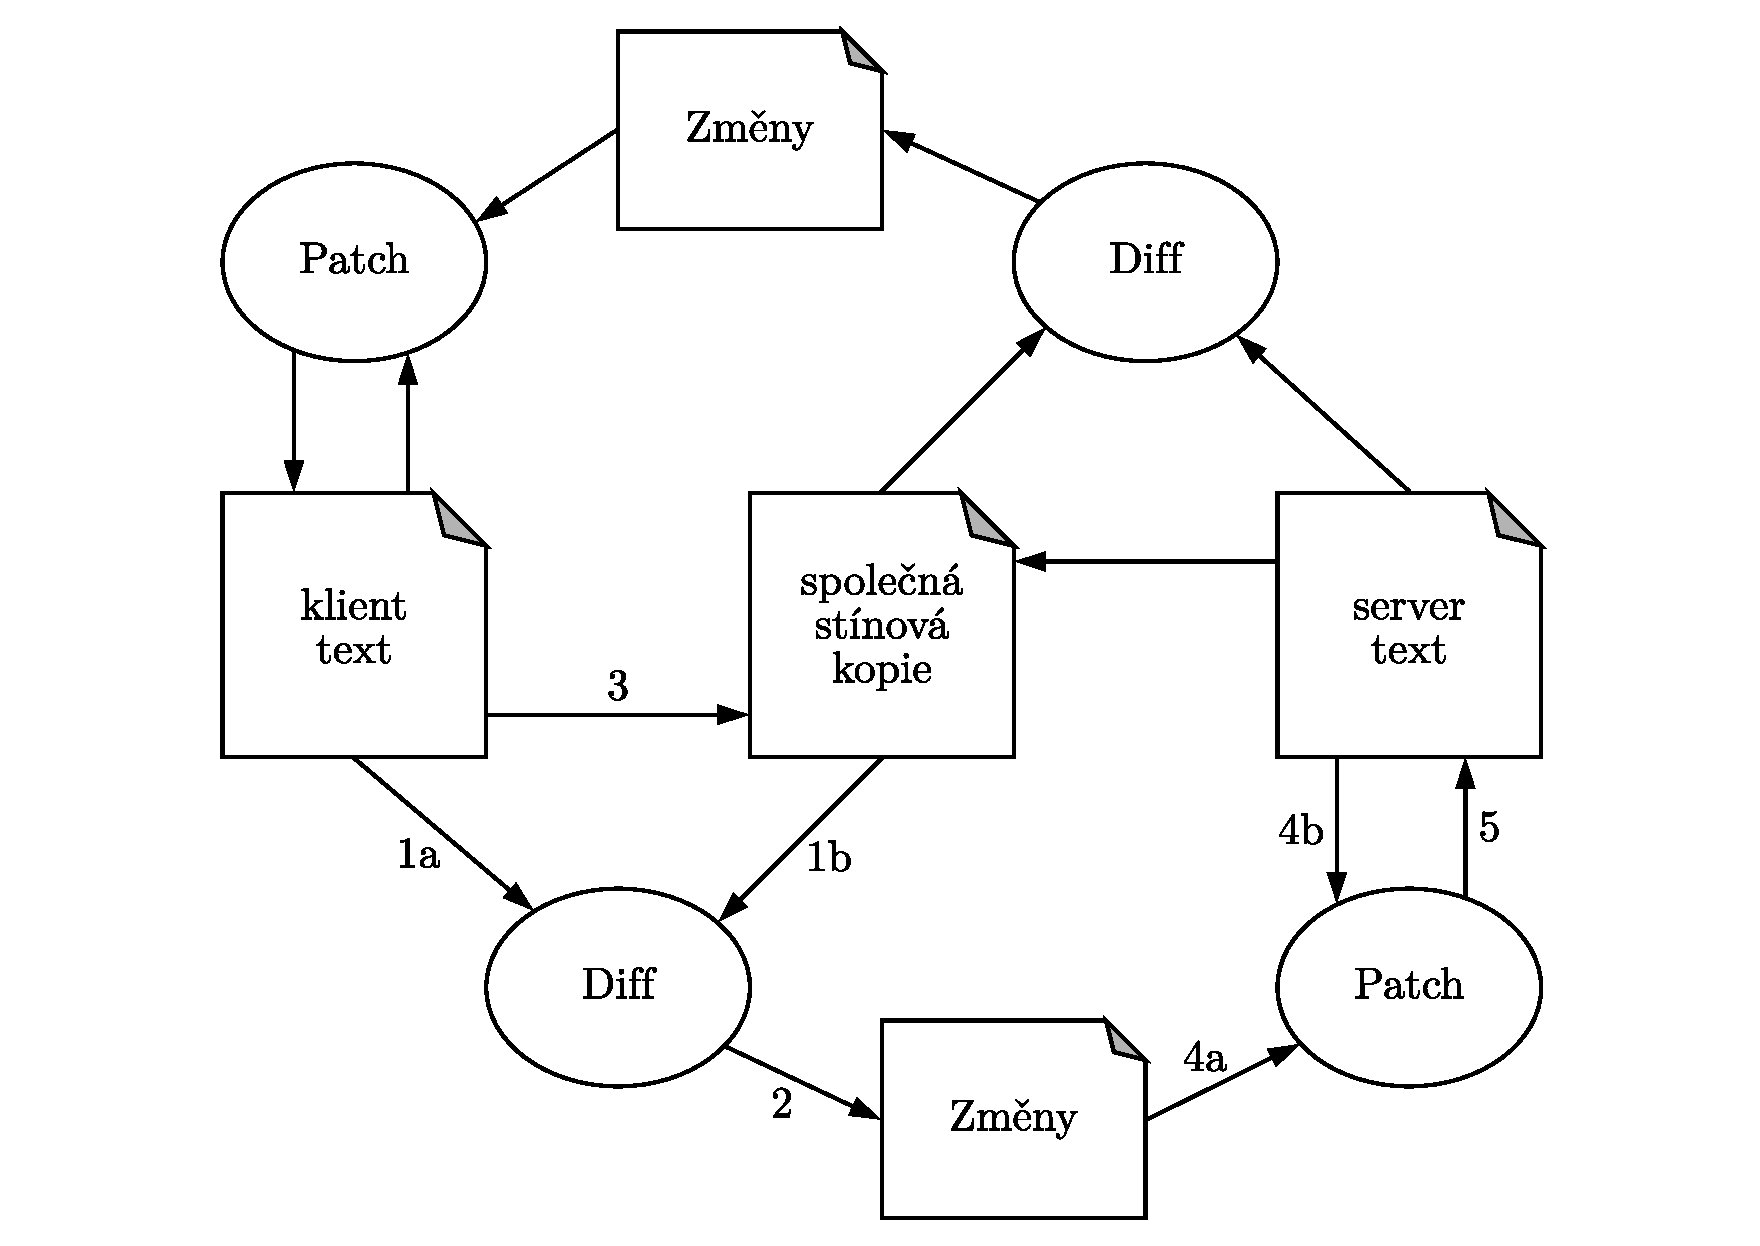
\includegraphics[width=\textwidth]{partials/analyza/DS_diagram.pdf}
    \caption{Diferenciální synchronizace vývojový diagram~\cite{ds:neil_paper}}\label{fig:DS_diagram}
\end{figure}

Na začátku jsou všechny dokumenty stejné (klient text, server text i společná stínová kopie).
Klient text i server text mohou být libovolně upraveny a cílem algoritmu je udržet oba dokumenty neustále co nejvíce podobné.

Algoritmus pokračuje následujícími kroky (viz čísla u jednotlivých přechodů diagramu~\ref{fig:DS_diagram}):
\begin{enumerate}
    \item \texttt{klient text} je porovnán oproti \texttt{společné stínové kopii},
    \item výsledkem porovnání je seznam změn, které byly provedeny na \texttt{klient text} kopii dokumentu,
    \item \texttt{klient text} je překopírován přes \texttt{společnou stínové kopii},
    \item seznam změn je aplikován na \texttt{server text} (za použití best-effort match algoritmu),\label{krok:ds_aplikace}
    \item \texttt{server text} je přepsán výsledkem aplikace změn.\label{krok:ds_prepsani}
\end{enumerate}

Důležité je, že pro správné fungování musí být kroky~\ref{krok:ds_aplikace} a~\ref{krok:ds_prepsani} atomické, tedy nesmí se stát, že by se server text v tuto chvíli změnil.

Algoritmus předpokládá použití libovolného diff-patch algoritmu, který umožňuje aplikovat změny i na dokument, který se změnil.
Lze například použít diff-match-patch algoritmus od společnosti Google.
Ten implementuje diff algoritmus od Eugene W. Myers, který je považování za nejlepší obecně použitelný diff algoritmus~\cite{ds:myers_diff}.~\cite{ds:neil_paper}~\cite{ds:neil_video}

\subsection{Operační transformace}\label{subsec:operacniTransformace}

\gls{OT} je algoritmus, který se poprvé objevil ve výzkumném článku s názvem Kontrola souběhu v skupinových systémech od autorů Ellis a Gibbs roku 1989.
Jedná se o nejčastěji používaný algoritmus pro kolaborativní editaci ve skutečném čase.~\cite{ot:intro}

Algoritmus je možné použít pro synchronizaci dokumentů různých formátů, ale pro jednoduchost se zaměřím pouze na textové dokumenty bez jakýchkoliv formátovacích značek (například zdrojový kód).

Základní jednotkou celého algoritmu je \textbf{operace}.
Operace označuje změnu v dokumentu a u čistě textových dokumentů rozlišujeme tři druhy operací:
\begin{itemize}
    \item přeskoč s parametrem počet znaků, který označuje počet znaků k přeskočení,
    \item odstraň řetězec s řetězcem jako parametrem, který označuje řetězec k odstranění,
    \item přidej řetězec s parametrem který označuje řetězec k přidání.~\cite{ot:aboutOT}
\end{itemize}

\paragraph{Transformace dokumentu}
Pomocí těchto třech operací lze popsat jakoukoli změnu, která mohla v dokumentu nastat, a zároveň daný dokument upravit, tak aby odpovídal stavu po této operaci.
Tento proces aplikace operace (či jejich souboru) se nazývá transformace dokumentu a umožňuje upravit dokument bez nutnosti jeho uzamčení, či řešení konfliktů.

Transformace má i své omezení, které říká, že součet znaků všech operací transformace se musí rovnat délce dokumentu, nad kterým bude transformace provedena.
Toto omezení není například u aplikace změn v rámci algoritmu \gls{DS} vůbec potřeba, protože změny nenesou informaci o délce celého dokumentu.

\paragraph{Kombinace operací}
Operace lze také kombinovat, určitě totiž platí, že je-li dám dokument A, soubor operací transformující dokument A na B a soubor operací transformující dokument B na C, tak jistě existuje soubor operací transformující dokument A na dokument C.

\paragraph{Transformace operací}
Dále lze operace transformovat a to pomocí jiných operací.
Je-li dán dokument A, soubory operací z A do B, z A do C, pak aplikací změn, z kterých byl vytvořen druhý soubor, na dokument B získáme nový soubor operací (soubor transformovaný).~\cite{ot:codecommit}


Základní komunikace se skládá z následujících kroků (také znázorněna pomocí sekvenčního diagramu na obrázku číslo~\ref{fig:OP_diagram}):

\begin{enumerate}
    \item po změně dokumentu klient změnu popíše pomocí souboru operací, který odešle na server,\label{krok:op_zmena}
    \item klient do přijetí potvrzení nesmí na server odeslat další operace, další změny si klient ukládá a kombinuje do jednoho velkého souboru operací,\label{krok:op_kombinace}
    \item server po přijetí odešle klientu, který soubor vytvořil, potvrzení o přijetí přijetí a pošle soubor všem ostatním klientům,
    \item klient po přijetí souboru může odeslat nastřádaný soubor zkombinovaných operací (pokračuje bodem~\ref{krok:op_kombinace}) nebo čeká na další změnu a pokračuje znovu bodem~\ref{krok:op_zmena}.~\cite{ot:waveAddition}
\end{enumerate}

\begin{figure}[ht]
    \centering
    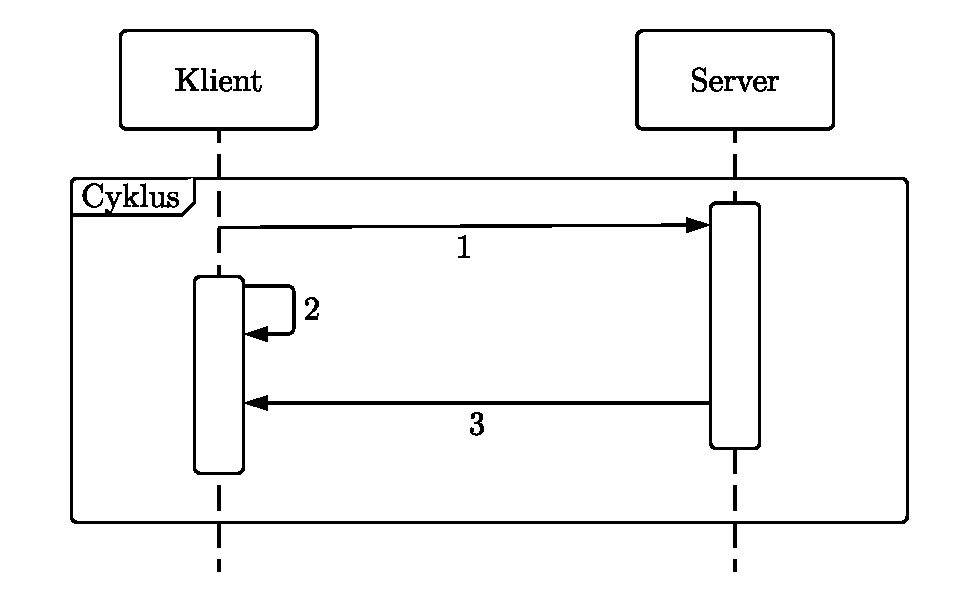
\includegraphics[width=\textwidth]{partials/analyza/OP_diagram.pdf}
    \caption{Operační transformace sekvenční diagram}\label{fig:OP_diagram}
\end{figure}

O čekání klienta před odesláním dalších operací na potvrzení přijetí posledního souboru serverem se zaručili vývojáři společnosti Google, kteří toto pravidlo poprvé použili pro službu Google Wave (více o službě v sekci~\ref{subsec:apacheWave}).
Toto vylepšení snižuje náročnost celého algoritmu omezením počtu současných operací, které by musel server kombinovat.~\cite{ot:waveAddition}

Pokud klient při čekání na potvrzení od serveru dostane cizí soubor operací, musí tento soubor aplikovat na svou kopii dokumentu a transformovat již uložené operace v závislosti na přijatých operacích.
Také pokud server dostane od klienta soubor operací, který vznikl před potvrzením posledního souboru, musí soubor transformovat přes všechny soubory operací, které server potvrdil po jeho vytvoření.
Z tohoto důvodu jsou soubory operací číslovány a klient s novým souborem operací odesílá na server i poslední pro něj známé číslo souboru.

Implementace obecného algoritmu \gls{OT} pro různé typy dokumentů není vůbec jednoduchá, což potvrzuje i následující tvrzení tehdejšího vývojáře Google Wave Josepha Gentle:

\enquote{\textit{Naneštěstí, implementovat OT není vůbec veselé.
Existuje milion algoritmů s různými kompromisy, které jsou však většinou uvězněny ve věděckých pracích.
Tyto algoritmy je opravdu obtížné a časově náročné správně implementovat.
[\ldots]
Jsem bývalý vývojář Google Wave.
Napsání Wave trvalo 2 roky a pokud bychom ho dnes chtěli přepsat, napodruhé by to trvalo téměř stejně tak dlouho.}}~\cite{ot:sharejs} přeložil Jiří Šimeček
